\section{Phân tích bài toán}

\subsection{Bài toán đặt ra}
Thương mại điện tử thời trang hiện nay đối mặt với tỷ lệ hoàn trả hàng cao do người mua không thể ước lượng chính xác kích thước và diện mạo trang phục khi mặc thực tế. Đề tài đặt ra bài toán xây dựng hệ thống thương mại điện tử tích hợp hai chức năng thử đồ ảo: Thử đồ thời gian thực qua camera sử dụng AR và ghép ảnh thử đồ tĩnh sử dụng AI để người dùng có thể xem trước trang phục trước khi mua.

\subsection{Các chức năng chính cần giải quyết}
\begin{itemize}
    \item \textbf{Thử đồ AR thời gian thực:} Nhận diện và theo dõi cơ thể người dùng qua camera, hiển thị mô hình 3D quần áo khớp với chuyển động cơ thể theo thời gian thực trên trình duyệt web.
    \item \textbf{Ghép ảnh thử đồ tĩnh:} Nhận ảnh người dùng và ảnh sản phẩm, sinh ra ảnh kết quả thể hiện người dùng mặc trang phục đó một cách chân thực bằng mô hình AI.
    \item \textbf{Gợi ý size:} Dựa trên thông số cơ thể người dùng, hệ thống tự động gợi ý kích thước phù hợp cho từng sản phẩm.
    \item \textbf{Tư vấn thời trang:} Chatbot sử dụng RAG và LLM để tư vấn sản phẩm phù hợp với nhu cầu người dùng.
\end{itemize}

\section{Các phương pháp thử đồ ảo}

\subsection{Tổng quan các phương pháp}
Hiện nay có hai hướng tiếp cận chính cho bài toán thử đồ ảo:

\begin{table}[H]
\centering
\begin{tabular}{|p{3cm}|p{5cm}|p{5cm}|}
\hline
\textbf{Tiêu chí} & \textbf{AR thời gian thực} & \textbf{AI ghép ảnh tĩnh} \\
\hline
Đầu vào & Camera trực tiếp & Ảnh người + ảnh quần áo \\
\hline
Tốc độ & Thời gian thực (realtime) & Vài giây đến vài phút \\
\hline
Độ chân thực & Trung bình (3D model) & Cao (AI sinh ảnh) \\
\hline
Thiết bị & Cần camera, GPU & Không cần camera \\
\hline
Ứng dụng & Xem trước nhanh & Xem chi tiết trước mua \\
\hline
\end{tabular}
\caption{So sánh hai phương pháp thử đồ ảo}
\end{table}

\subsection{Phương pháp AR thời gian thực}
Phương pháp này sử dụng camera để nhận diện cơ thể người dùng và overlay mô hình 3D quần áo lên. Hình \ref{fig:ar_pipeline} mô tả pipeline xử lý gồm 5 bước chính:

\begin{figure}[H]
\centering
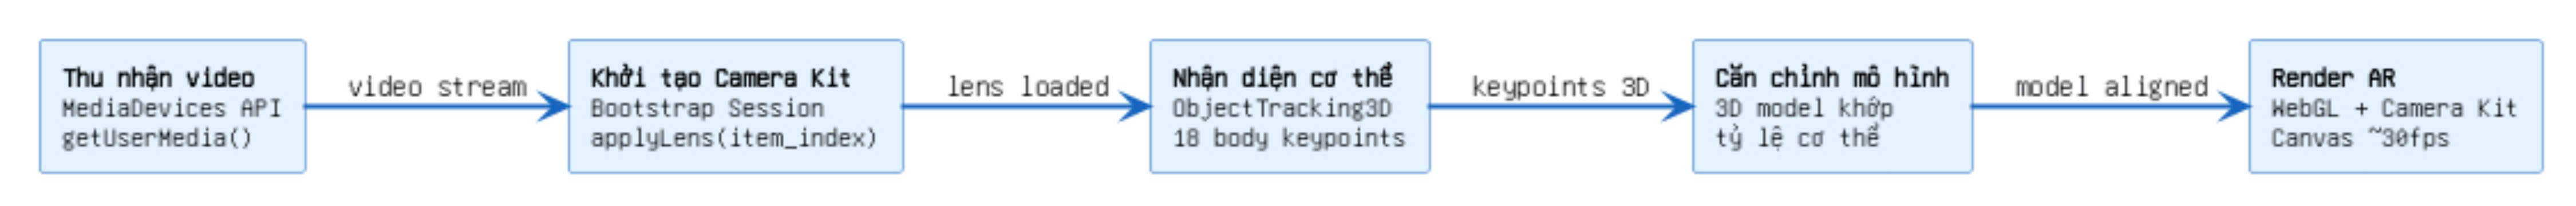
\includegraphics[width=\textwidth]{graphics/main/chapter1/PipeAR.jpg}
\caption{Pipeline xử lý AR thời gian thực}
\label{fig:ar_pipeline}
\end{figure}

\begin{enumerate}
    \item \textbf{Thu nhận video:} Camera thu hình ảnh người dùng liên tục thông qua MediaDevices API với lệnh getUserMedia(), tạo ra luồng video đầu vào cho hệ thống.
    \item \textbf{Khởi tạo Camera Kit:} Camera Kit Web SDK khởi tạo phiên làm việc (Bootstrap Session) và nạp Lens thông qua applyLens(), truyền tham số item\_index để xác định mô hình quần áo cần hiển thị.
    \item \textbf{Nhận diện cơ thể:} Module ObjectTracking3D của Lens Studio phát hiện và theo dõi 18 keypoint cơ thể (vai, hông, tay, chân...) trong không gian 3D theo thời gian thực.
    \item \textbf{Căn chỉnh mô hình:} Mô hình 3D quần áo được căn chỉnh theo đúng tỷ lệ và vị trí cơ thể dựa trên các keypoint thu được từ bước trước.
    \item \textbf{Render AR:} Camera Kit render kết quả qua WebGL lên canvas trình duyệt với tốc độ khoảng 30fps, tạo ra trải nghiệm thử đồ thời gian thực mượt mà.
\end{enumerate}

\noindent\textbf{Ưu điểm:} Phản hồi tức thì, tương tác tự nhiên, không cần ảnh đầu vào.

\noindent\textbf{Nhược điểm:} Độ chân thực thấp hơn AI, phụ thuộc vào chất lượng camera và ánh sáng.

\subsection{Phương pháp AI ghép ảnh tĩnh}
Phương pháp này sử dụng mô hình học sâu để ghép ảnh quần áo lên ảnh người dùng.
Bảng \ref{tab:vton_compare} so sánh các kiến trúc phổ biến hiện nay:

\begin{table}[H]
\centering
\begin{tabular}{|p{3cm}|p{3.5cm}|p{3.5cm}|p{2.5cm}|}
\hline
\textbf{Kiến trúc} & \textbf{Ưu điểm} & \textbf{Nhược điểm} & \textbf{Đại diện} \\
\hline
GAN-based & Tốc độ nhanh, nhẹ & Hay bị artifact, kém tự nhiên & VITON, HR-VITON \\
\hline
Flow-based & Bảo toàn kết cấu vải tốt & Khó xử lý biến dạng lớn & ClothFlow \\
\hline
Diffusion-based & Chất lượng cao nhất, tự nhiên, bảo toàn texture & Thời gian xử lý lâu hơn & FitDiT, CatVTON \\
\hline
\end{tabular}
\caption{So sánh các kiến trúc Virtual Try-On}
\label{tab:vton_compare}
\end{table}

Đề tài lựa chọn FitDiT thuộc nhóm Diffusion-based vì cho chất lượng ảnh cao nhất, bảo toàn chi tiết texture vải và xử lý tốt các tư thế phức tạp, phù hợp với yêu cầu thử đồ chân thực trước khi mua hàng.

Pipeline xử lý của phương pháp AI được mô tả trong Hình \ref{fig:ai_pipeline}:

\begin{figure}[H]
\centering
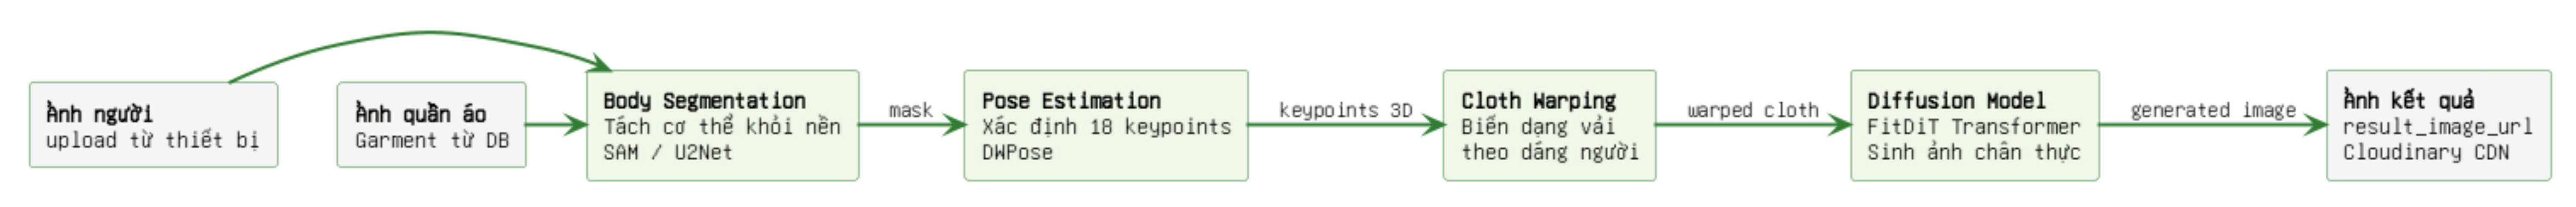
\includegraphics[width=\textwidth]{graphics/main/chapter1/PipeAI.jpg}
\caption{Pipeline xử lý AI ghép ảnh thử đồ (FitDiT)}
\label{fig:ai_pipeline}
\end{figure}

\begin{enumerate}
    \item \textbf{Đầu vào:} Hệ thống nhận hai đầu vào song song: ảnh người dùng upload từ thiết bị và ảnh quần áo lấy từ cơ sở dữ liệu (Garment DB).
    \item \textbf{Phân đoạn cơ thể (Body Segmentation):} Mô hình SAM/U2Net tách vùng cơ thể khỏi nền ảnh, tạo ra mask cơ thể làm cơ sở cho các bước tiếp theo.
    \item \textbf{Ước lượng tư thế (Pose Estimation):} Module DWPose xác định 18 keypoint cơ thể, cung cấp thông tin tư thế để căn chỉnh quần áo chính xác theo dáng người.
    \item \textbf{Warping quần áo (Cloth Warping):} Ảnh quần áo được biến dạng (warp) theo dáng và tư thế cơ thể người dùng dựa trên keypoint thu được.
    \item \textbf{Sinh ảnh kết quả (Diffusion Model):} FitDiT Transformer tổng hợp ảnh cuối cùng, kết hợp người và quần áo một cách tự nhiên với độ chân thực cao.
    \item \textbf{Đầu ra:} Ảnh kết quả được lưu lên Cloudinary CDN và trả về đường dẫn ảnh để hiển thị cho người dùng.
\end{enumerate}

Trong hệ thống thực tế, FitDiT được tích hợp theo mô hình xử lý async: Frontend gửi yêu cầu tới Backend (FastAPI), Backend tạo job và trả về mã định danh job ngay lập tức, sau đó Frontend tự động kiểm tra trạng thái mỗi 5 giây cho đến khi nhận được ảnh kết quả. Cách tiếp cận này giúp tránh timeout do thời gian xử lý của mô hình AI có thể kéo dài từ 30 giây đến vài phút tùy độ phức tạp của ảnh đầu vào.

\noindent\textbf{Ưu điểm:} Độ chân thực cao, bảo toàn chi tiết vải, không cần camera.

\noindent\textbf{Nhược điểm:} Thời gian xử lý lâu hơn AR, cần ảnh đầu vào chất lượng tốt.

\subsection{Chức năng gợi ý size}
Hệ thống gợi ý size dựa trên thông số cơ thể người dùng (chiều cao, cân nặng, số đo vòng ngực/eo/hông) được lưu trong \textbf{Body Profile} tại cơ sở dữ liệu Neon PostgreSQL, kết hợp với bảng size chuẩn của từng sản phẩm do người bán nhập vào. Pipeline xử lý được mô tả trong Hình \ref{fig:size_pipeline}:

\begin{figure}[H]
\centering
\begin{tikzpicture}[
    node distance=0.6cm,
    box/.style={rectangle, rounded corners=6pt, draw=orange!70!black, fill=orange!8,
                text width=3.5cm, align=center, minimum height=1cm, font=\small},
    arrow/.style={-{Stealth[length=3mm]}, thick, orange!70!black}
]
\node[box] (A) {\textbf{Nhập thông số}\\{\footnotesize Chiều cao, cân nặng,\\số đo cơ thể}};
\node[box, right=of A] (B) {\textbf{Tra bảng size}\\{\footnotesize So sánh với\\bảng size sản phẩm}};
\node[box, right=of B] (C) {\textbf{Tính toán}\\{\footnotesize Đánh giá mức độ\\phù hợp}};
\node[box, right=of C] (D) {\textbf{Gợi ý size}\\{\footnotesize Vừa khít / Rộng\\/ Chật}};
\draw[arrow] (A) -- (B);
\draw[arrow] (B) -- (C);
\draw[arrow] (C) -- (D);
\end{tikzpicture}
\caption{Pipeline gợi ý size trang phục}
\label{fig:size_pipeline}
\end{figure}

\begin{enumerate}
    \item \textbf{Nhập thông số:} Người dùng nhập hoặc cập nhật thông số cơ thể (chiều cao, cân nặng, vòng ngực, vòng eo, vòng hông) trong trang hồ sơ cá nhân. Dữ liệu được lưu vào bảng body\_profiles trong cơ sở dữ liệu Neon PostgreSQL.
    \item \textbf{Tra bảng size:} Hệ thống truy vấn bảng garment\_sizes tương ứng với sản phẩm, so sánh từng số đo của người dùng với ngưỡng tối thiểu và tối đa của từng size (S, M, L, XL...).
    \item \textbf{Tính toán mức độ phù hợp:} Backend đánh giá từng số đo theo ba mức: vừa khít (fit), rộng (loose) hoặc chật (tight), sau đó tổng hợp để đưa ra gợi ý size tối ưu.
    \item \textbf{Trả kết quả:} Hệ thống gợi ý size phù hợp kèm mức độ đánh giá cho từng số đo (ngực, eo, hông), giúp người dùng hiểu rõ lý do và tự quyết định size phù hợp nhất.
\end{enumerate}
\subsection{Lựa chọn của đề tài}
Đề tài kết hợp cả ba phương pháp để tận dụng ưu điểm của từng hướng, tạo ra trải nghiệm mua sắm toàn diện cho người dùng:

\begin{itemize}
    \item \textbf{AR thời gian thực (Snap Camera Kit và Lens Studio):} Cho phép người dùng xem nhanh trang phục qua camera ngay trên trang sản phẩm, tạo trải nghiệm tương tác tức thì mà không cần chuẩn bị ảnh đầu vào.
    \item \textbf{AI ghép ảnh (FitDiT):} Cho phép người dùng upload ảnh cá nhân để xem kết quả thử đồ chi tiết, chân thực hơn trước khi quyết định mua.
    \item \textbf{Gợi ý size tự động:} Dựa trên thông số cơ thể người dùng kết hợp bảng size sản phẩm, hệ thống gợi ý size phù hợp kèm mức độ đánh giá, giúp giảm thiểu tỷ lệ hoàn trả hàng do chọn sai kích thước.
\end{itemize}